\documentclass[11pt]{article}
%-----------Packeges---------------%
\usepackage{amsmath}
\usepackage{amssymb}
\usepackage{amsfonts}
\usepackage{tocloft}
\usepackage{float}
\usepackage{graphicx}
\usepackage[bookmarks=true]{hyperref}
\usepackage{fancyhdr}


%----------Definition & Theorem----%
\newtheorem{definition}{Definition}[subsection]
\newtheorem{theorem}{Theorem}[subsection]
\newtheorem{proposition}{Proposition}[subsection]
\newtheorem{lemma}{Lemma}[subsection]
\newtheorem{corollary}{Corollary}[subsection]

\pagestyle{fancy}
\fancyhead[L]{CS 412}
\fancyhead[C]{HW5}
\fancyhead[R]{Lanxiao Bai}

\usepackage{listings}
\usepackage{color}
\usepackage{enumerate}
\usepackage{tikz}

\definecolor{dkgreen}{rgb}{0,0.6,0}
\definecolor{gray}{rgb}{0.5,0.5,0.5}
\definecolor{mauve}{rgb}{0.58,0,0.82}

\lstset{frame=tb,
  language=Python,
  aboveskip=3mm,
  belowskip=3mm,
  showstringspaces=false,
  columns=flexible,
  basicstyle={\small\ttfamily},
  numbers=none,
  numberstyle=\tiny\color{gray},
  keywordstyle=\color{black},
  commentstyle=\color{dkgreen},
  stringstyle=\color{black},
  breaklines=true,
  breakatwhitespace=true,
  tabsize=3
}

\begin{document}
	\begin{enumerate}
		\item 
		\begin{enumerate}[a.]
			\item 
			\begin{enumerate}[i.]
				\item \[Pr(\text{Popularity = 'P'}) = \frac{N(\text{Popularity = 'P'})}{N_{total}} = \frac{7}{10} \]
				\item \[Pr(\text{Popularity = 'NP'}) = 1 - Pr(\text{Popularity = 'P'}) = \frac{3}{10}\]
				\item \[Pr\text{('\$', 'Yes' , 'Korean' $|$ 'P')}\\ = \frac{0 + 1}{7 + 2} = \frac{1}{9}\]
				\item \[Pr\text{('\$', 'Yes' ,'Korean' $|$ 'NP')}\\ = \frac{0 + 1}{3 + 2} = \frac{1}{5}\]
			\end{enumerate}
			\item 
			\begin{align}
				&\phantom{ =\ \ }Pr(\text{Popularity = 'P' $|$ Price = '\$', Delivery = 'Yes' , Cuisine = 'Korean'})\nonumber\\
				&=\frac{Pr(\text{\$, Yes, Korean $|$ P})Pr(\text{P})}{Pr(\text{\$, Yes, Korean})}\nonumber\\
				&=\frac{Pr(\text{\$ $|$ P})Pr(\text{Yes $|$ P})Pr(\text{Korean $|$ P})Pr(\text{P})}{Pr(\text{\$, Yes, Korean})}\nonumber\\
				&=\frac{Pr(\text{\$ $|$ P})Pr(\text{Yes $|$ P})Pr(\text{Korean $|$ P})Pr(\text{P})}{Pr(\text{\$, Yes, Korean $|$ P})Pr(\text{P}) + Pr(\text{\$, Yes, Korean $|$ NP})Pr(\text{NP})}\nonumber\\
				&= \frac{4/7 \cdot 4/7 \cdot 2/7 \cdot 7/10}{1/9 \cdot 7/10 + 1/5 \cdot 3/10}\nonumber\\
				&= \frac{720}{1519} \approx 0.474\nonumber
			\end{align}
			
			\begin{align}
				&\phantom{ =\ \ }Pr(\text{Popularity = 'NP' $|$ Price = '\$', Delivery = 'Yes' , Cuisine = 'Korean'})\nonumber\\
				&=\frac{Pr(\text{\$, Yes, Korean $|$ NP})Pr(\text{NP})}{Pr(\text{\$, Yes, Korean})}\nonumber\\
				&=\frac{Pr(\text{\$ $|$ NP})Pr(\text{Yes $|$ NP})Pr(\text{Korean $|$ NP})Pr(\text{NP})}{Pr(\text{\$, Yes, Korean})}\nonumber\\
				&=\frac{Pr(\text{\$ $|$ NP})Pr(\text{Yes $|$ NP})Pr(\text{Korean $|$ NP})Pr(\text{NP})}{Pr(\text{\$, Yes, Korean $|$ P})Pr(\text{P}) + Pr(\text{\$, Yes, Korean $|$ NP})Pr(\text{NP})}\nonumber\\
				&= \frac{1/3 \cdot 2/3 \cdot 1/3 \cdot 3/10}{1/9 \cdot 7/10 + 1/5 \cdot 3/10}\nonumber\\
				&= \frac{5}{31} \approx 0.1613\nonumber
			\end{align}
			
			Since $Pr(\text{Popularity = 'P' $|$ Price = '\$', Delivery = 'Yes' , Cuisine = 'Korean'}) > Pr(\text{Popularity = 'NP' $|$ Price = '\$', Delivery = 'Yes' , Cuisine = 'Korean'})$, we classify this tuple as \textbf{popular}.
			\item We can train $n$ Naive Bayes classifiers each with randomly sampled data from the original dataset and make decision by majority vote.
			\item Since the number of positive samples are small, we want to make sure that the naive Bayes classifier just label all data as negative, thus, we choose
			\[\text{Recall} = \frac{\text{True positive}}{\text{True positive} + \text{False negative}}\]
			
			to be our metric.
		\end{enumerate}
		\item By running the code in 
			\begin{enumerate}[a.]
				\item Since the indices of closest points are $5, 1, 4, 7$ when $K = 1$, so the predictions are $-1, 1, -1, -1$. Testing error when $K = 1$ is $error = 0.25$.
				\item Since the indices of closest points are $[5, 2, 3], [1, 2, 3], [4, 6, 5], [7, 0, 1]]$ when $K = 3$, so the predictions are $1, 1, -1, 1$. Testing error when $K = 3$ is $error = 0.25$.
				\item By using SGD to fit the model, we get $a = 12.452, b = -11.991, c = -0.106$ and training error is $0$ and testing error is $0.25$.
				\item KNN is very sensitive to outliers comparing to linear model, KNN requires more space to store the training data while linear model only stores the weights, KNN takes more time to evaluate.
			\end{enumerate}
			\item 
			\begin{enumerate}[a.]
				\item
				Iteration 1:

	$d1 = 1.414214 \leq d2 = 5.385165$, $(1, 3)$ in cluster 1

	$d1 = 2.236068 \leq d2 = 5.830952$, $(1, 2)$ in cluster 1

	$d1 = 3.605551 \leq d2 = 5.656854$, $(2, 1)$ in cluster 1

	$d1 = 2.828427 \leq d2 = 5.000000$, $(2, 2)$ in cluster 1

	$d1 = 2.236068 \leq d2 = 4.472136$, $(2, 3)$ in cluster 1

	$d1 = 3.605551 \leq d2 = 4.242641$, $(3, 2)$ in cluster 1

	$d1 = 5.099020 > d2 = 2.236068$, $(5, 3)$ in cluster 2

	$d1 = 4.123106 > d2 = 2.828427$, $(4, 3)$ in cluster 2

	$d1 = 4.123106 > d2 = 2.000000$, $(4, 5)$ in cluster 2

	$d1 = 5.000000 > d2 = 1.414214$, $(5, 4)$ in cluster 2

	$d1 = 5.099020 > d2 = 1.000000$, $(5, 5)$ in cluster 2

	$d1 = 6.000000 > d2 = 1.000000$, $(6, 4)$ in cluster 2

	$d1 = 6.082763 > d2 = 0.000000$, $(6, 5)$ in cluster 2

	Center1 : (1, 2), Center2 : $(5, 4)$

Iteration 2:

	$d1 = 1.000000 \leq d2 = 4.123106$, $(1, 3)$ in cluster 1

	$d1 = 0.000000 \leq d2 = 4.472136$, $(1, 2)$ in cluster 1

	$d1 = 1.414214 \leq d2 = 4.242641$, $(2, 1)$ in cluster 1

	$d1 = 1.000000 \leq d2 = 3.605551$, $(2, 2)$ in cluster 1

	$d1 = 1.414214 \leq d2 = 3.162278$, $(2, 3)$ in cluster 1

	$d1 = 2.000000 \leq d2 = 2.828427$, $(3, 2)$ in cluster 1

	$d1 = 4.123106 > d2 = 1.000000$, $(5, 3)$ in cluster 2

	$d1 = 3.162278 > d2 = 1.414214$, $(4, 3)$ in cluster 2

	$d1 = 4.242641 > d2 = 1.414214$, $(4, 5)$ in cluster 2

	$d1 = 4.472136 > d2 = 0.000000$, $(5, 4)$ in cluster 2

	$d1 = 5.000000 > d2 = 1.000000$, $(5, 5)$ in cluster 2

	$d1 = 5.385165 > d2 = 1.000000$, $(6, 4)$ in cluster 2

	$d1 = 5.830952 > d2 = 1.414214$, $(6, 5)$ in cluster 2

	Center1 : (1, 2), Center2 : $(5, 4)$

Cluster 1: $[(1, 3), (1, 2), (2, 1), (2, 2), (2, 3), (3, 2)]$

Cluster 2: $[(5, 3), (4, 3), (4, 5), (5, 4), (5, 5), (6, 4), (6, 5)]$

	which means that Cluster 1 is  point 1 to 6 and Cluster 2 is point 7 to 13
	\item By checking the $\varepsilon$ neighborhood, we see that from any point in this dataset, we can always add the rest points into the cluster since they are all surrounded by more than $MinPts = 2$ points in the dataset, thus, we put points $1$ to $13$ into the same cluster.
	\item 
	By applying AGNES, we get the cluster hierarchy as following (next page)
		\begin{figure}[H]
			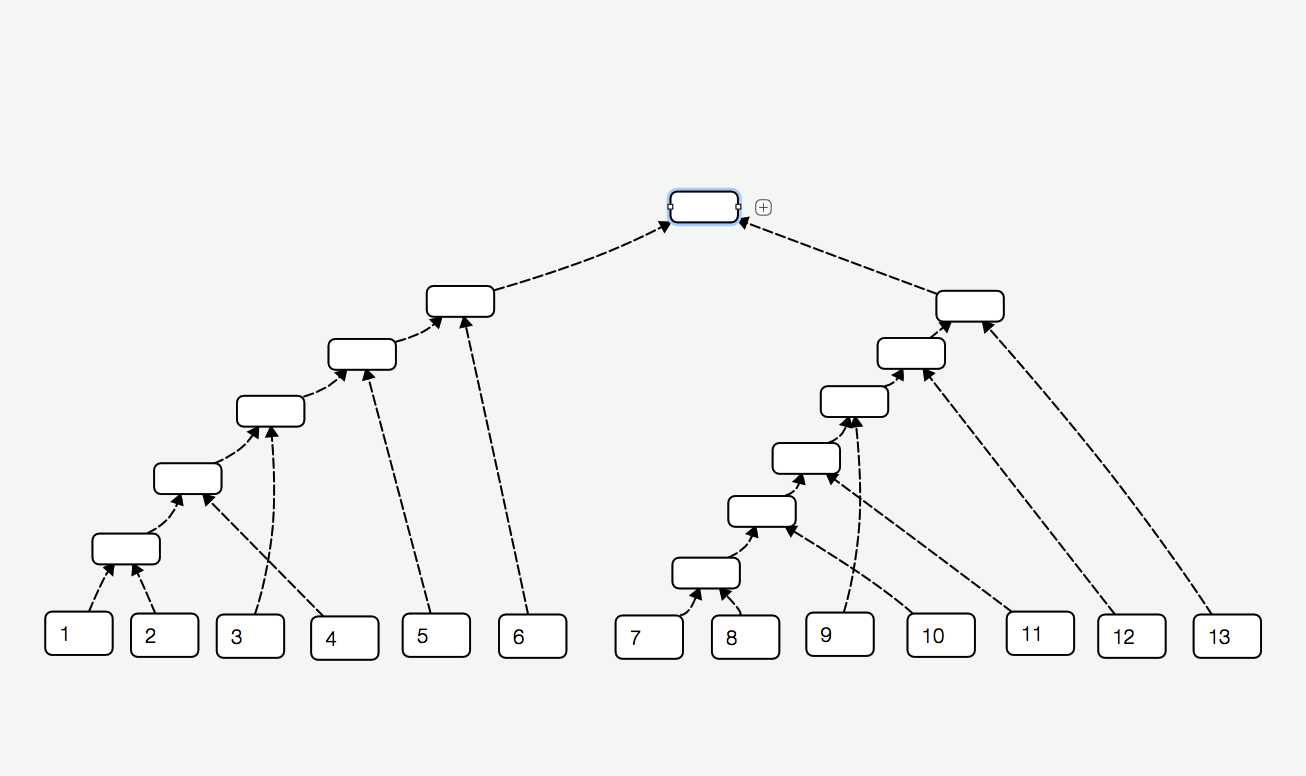
\includegraphics[width=\textwidth]{hierarchy}
			\caption{Result of applying AGNES on given dataset}
		\end{figure}
		\end{enumerate}
	\end{enumerate}
\end{document}